In graph theory, a \emph{walk} is a sequence of edges connected by vertices. A \emph{self-avoiding walk} is one that can be traced from start to finish without tracing over the same vertex more than once. Put another way, the a walk $w$ is self-avoiding if $w$ does not have any self loops.

A finite automaton can be used to process the set of edges $3\times n$ square lattice. We develop a set of symbols that can be used to encode any such lattice; this symbol set constitutes the input alphabet of the finite automaton that recognizes lattices that contain a self-avoiding walk.

This finite automata accepts square lattices that meet the following criteria:
\begin{enumerate}
\item The edges of the lattice represent a self-avoiding walk.
\begin{enumerate}
\item Walks in the lattice do not ``jump''; that is, there are exactly two ends, or vertices of degree 1.
\item Walks in the lattice do not ``branch''; that is, no vertex has degree greater than 2.
\item There are no closed loops in the lattice.
\end{enumerate}
\item A walk begins at the ``origin'' (the leftmost, bottom point) of the lattice. This condition not only simplifies the design of the automaton, but also ensures that if the automaton is used to count self-avoiding walks, double-counting the horizontal translations or vertical reflections of the same walk is avoided.
\end{enumerate}



\begin{figure}
\begin{center}
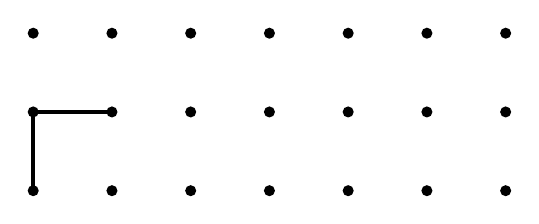
\begin{tikzpicture}
\foreach \x in {0,...,6}
\foreach \y in {0,1,2}
{
\fill (\x,\y) circle (2pt);
}
\draw [ultra thick] (0,0) -- (0,1) -- (1,1);
\end{tikzpicture}
\end{center}
\caption{PLACEHOLDER DOT MATRIX}
\end{figure}
